\ProvidesFile{ch1.tex}[Chapter1]

\chapter{SINGLE MOLECULE LOCALIZATION MICROSCOPY}
\ix{physics//Physics appendix}

\section{Introduction}

\subsection{Breaking the diffraction barrier}

In the quest to understand cellular function, biologists aim to directly observe the processes enabling cells to maintain homeostasis and respond dynamically to internal and environmental cues at the molecular level. However, the inherent limitations imposed by diffraction have historically constrained the resolution achievable with conventional light microscopy. The diffraction limit, first described by Ernst Abbe in the 19th century, dictates that the resolution of a microscope is fundamentally limited by the wavelength of light used for imaging. Objects closer than approximately half the wavelength of light cannot be distinguished as separate entities. For visible light, this translates to a resolution limit of about 200-250 nanometers, which is insufficient for resolving many subcellular structures and molecular complexes.

Super-resolution (SR) microscopy techniques have emerged as a pathway to observing subcellular structures and dynamics with enhanced resolution, surpassing the classical Abbe diffraction limit. Fluorescence microscopy techniques continually push the resolution boundary towards nanometer scales, facilitating imaging of cellular structures with a level of detail previously achievable only with electron microscopy. Concurrently, SR techniques retain the advantages of optical microscopy in biological experiments, including sample preservation, imaging flexibility, and target specificity. SR enables extraction of quantitative information on spatial distributions and often absolute numbers of proteins, nucleic acids, or other macromolecules within subcellular compartments.

A host of SR methods have been developed in recent years, which fundamentally differ in how fluorescently labeled samples are excited and how the emitted photons are detected. Here, we focus on a particular technique referred to as single-molecule localization microscopy or nanoscopy. This class of diffraction-unlimited SR methods leverage fluorescence intermittency to resolve fluorophores which would otherwise be unresolvable at the detector (Figure \ref{fig:fig1}). Nanoscopy approaches, such as direct-STORM (dSTORM), have become quite popular because they can be implemented at low cost on conventional wide-field setups, shifting the complexity to biological sample preparation and image post-processing. Common strategies for the temporal separation of molecules involve transient intramolecular rearrangements to switch from dark to fluorescent states, or the exploitation of non-emitting molecular radicals. For example, in dSTORM, rhodamine derivatives can undergo intersystem crossing to a triplet state, which can be reduced by thiols to form a dark radical species. The dark state can then be quenched by oxidative processes, driving the fluorophore back to its ground state. 

\begin{figure}[t]
\centering
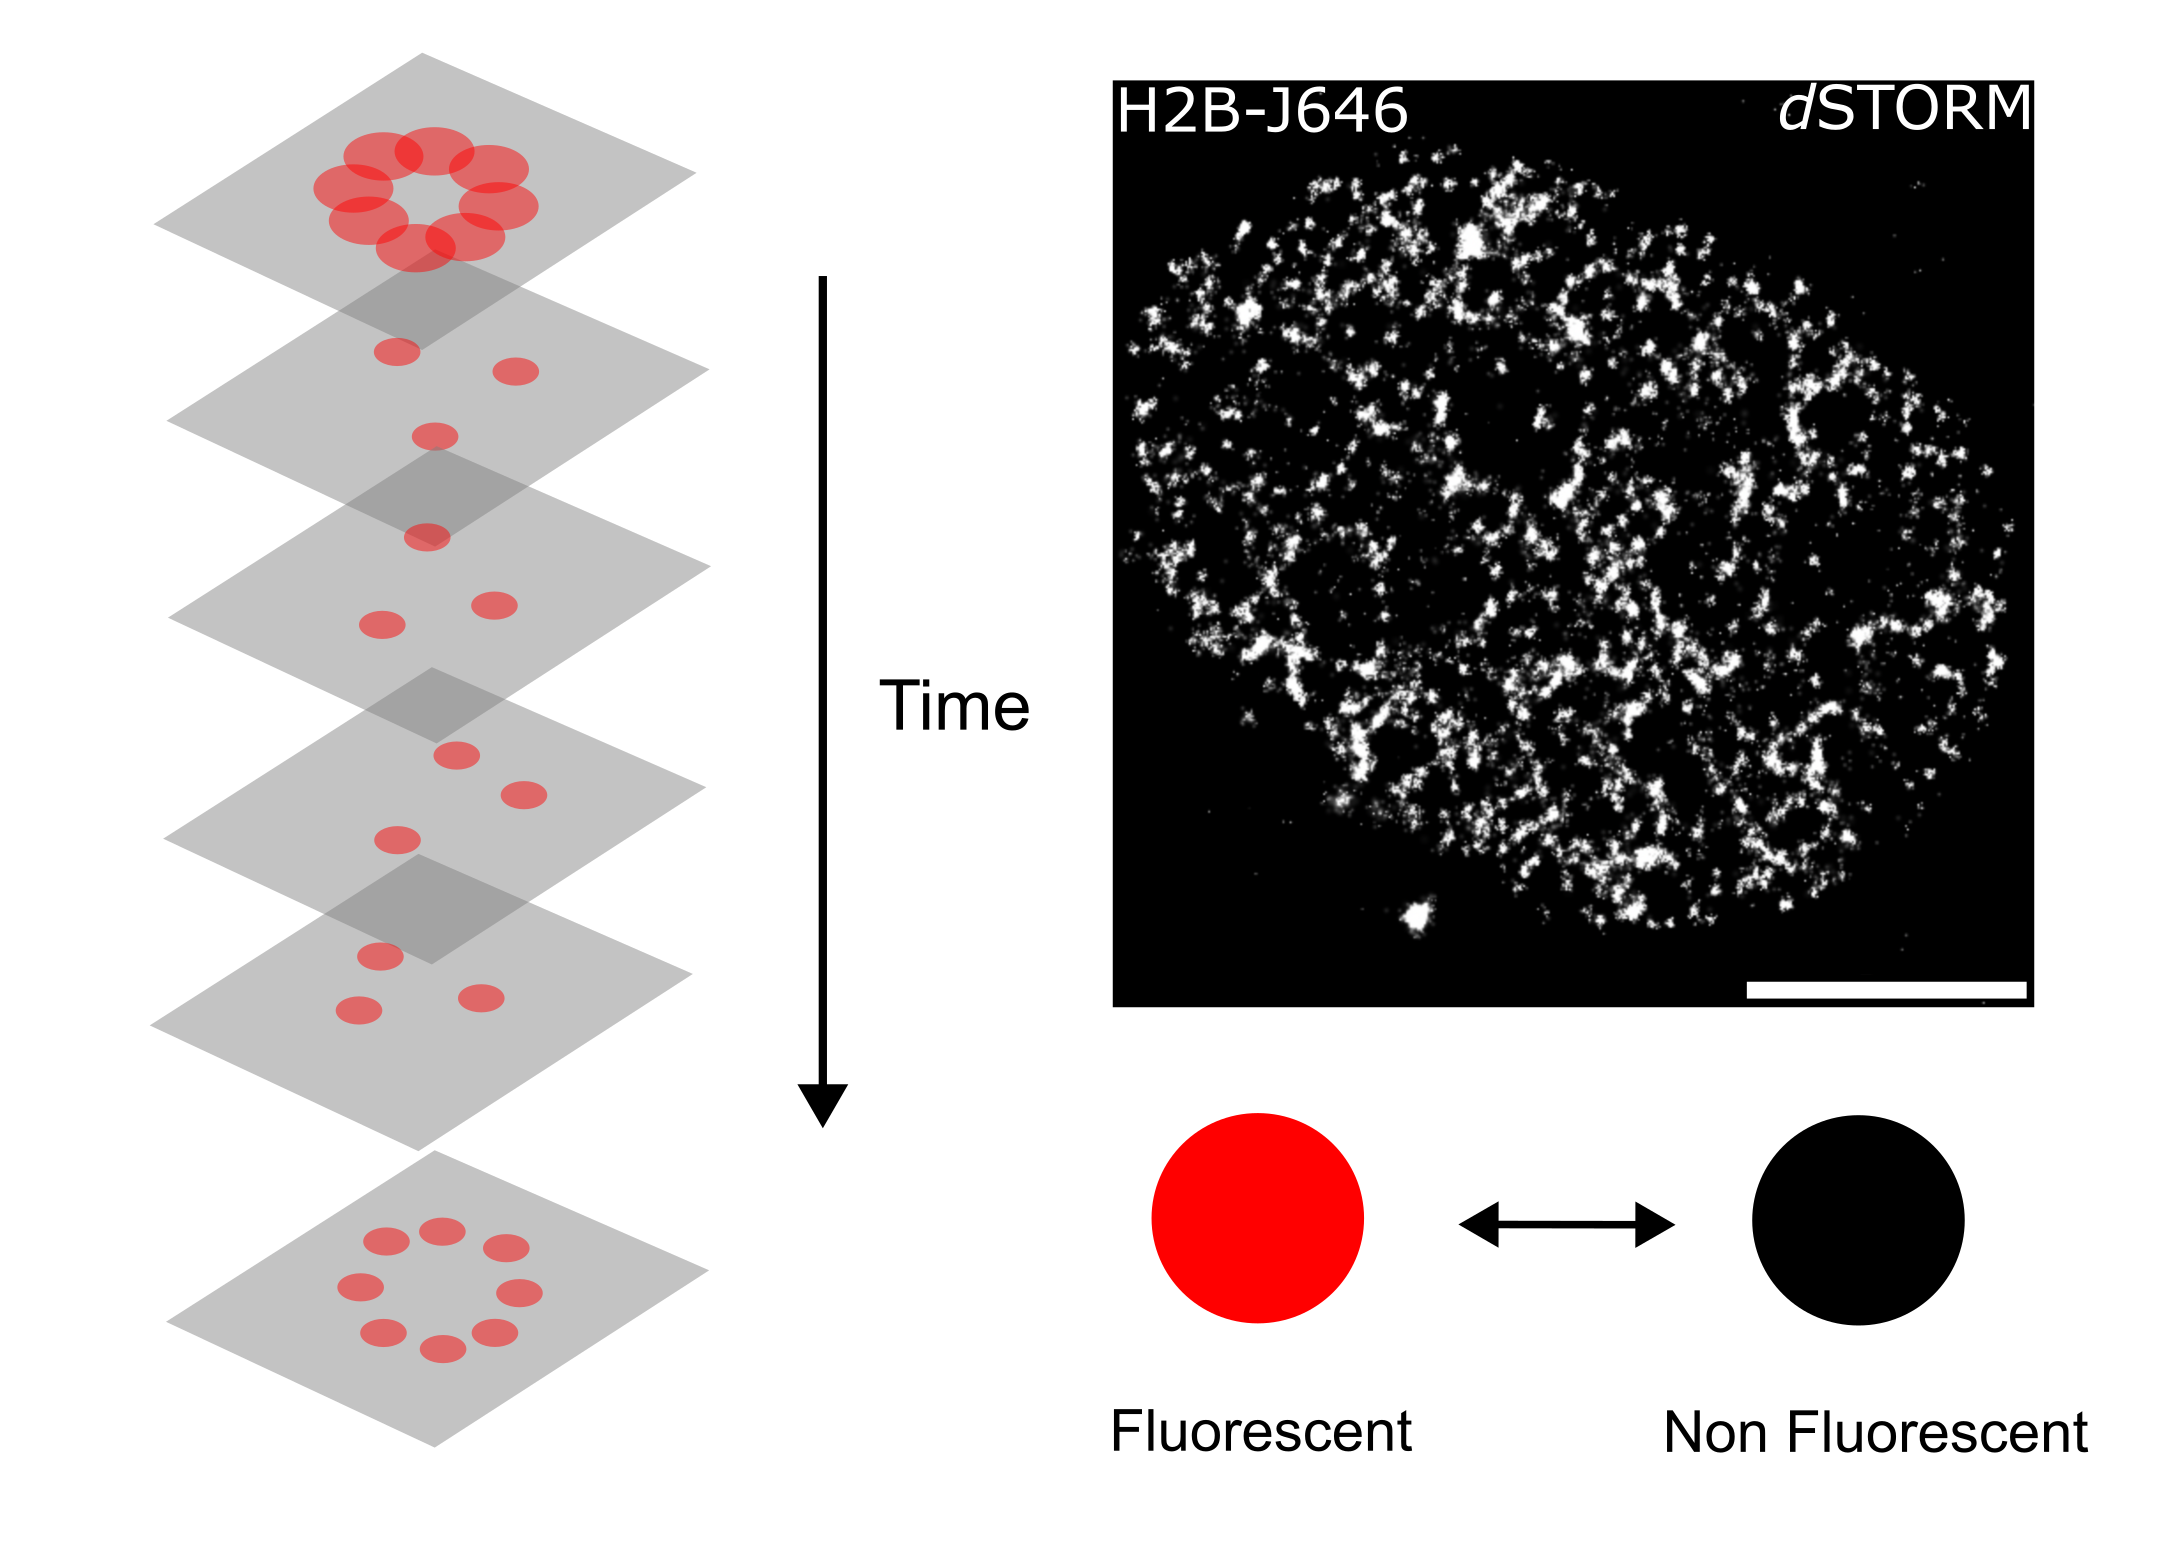
\includegraphics[width=11cm]{media/Intro.png}
\caption{\textbf{Stochastic optical reconstruction microscopy (STORM)}. Single molecules are resolved by separating their fluorescent emission in time using fluorophores with multiple photophysical states. Example super-resolution image of H2B protein in a living Hela cell nucleus at 37C, 5 percent CO2. Image reconstructed from 1k 10ms frames. Scalebar 5um.}
\label{fig:fig1}
\end{figure}

In nanoscopy applications, we seek the position and intensity of isolated fluorophores as well as estimate the accuracy and precision of these parameters. Accuracy is a measure of the systematic error or bias, and precision is a measure of the statistical error of an estimator. Both of these metrics are crucial in nanoscopy, as they determine the quality of SR reconstructions and maximum achievable resolution of the method, respectively. Importantly, a SR image in nanoscopy is simply a kernel density estimate (KDE) of the located fluorescent emitters, using an isotropic Gaussian kernel. The width of one such placed Gaussian kernel, $\sigma$ is given by the precision of the fluorophore position localization. The value of $\sigma$ will depend on experimental factors such as the signal-to-noise ratio (SNR). A fundamental lower bound on $\sigma$ is discussed in Section 1.2.1.

\subsection{Biological discovery with fluorescence nanoscopy}

Using fluorescence nanoscopy, scientists can now explore the nanoscale organization of cells and their components, leading to groundbreaking discoveries and new insights into cellular processes. In immunology, nanoscopy has been employed to study the spatiotemporal dynamics of T cell antigen receptor (TCR) complexes and linker for activation of T cells (LAT), an important adaptor molecule in the TCR signaling pathway \parencite{Lillemeier2010}. Others used nanoscopy to demonstrate that clustering patterns of the tyrosine kinase Lck were controlled by the conformational states of Lck, with the open, active conformation inducing clustering and the closed, inactive conformation preventing clustering \parencite{Rossy2013}. Nanoscopy has also proven invaluable in virology. In this field, researchers have utilized nanoscopy techniques to visualize Human immunodeficiency virus type 1 (HIV-1) assembly and budding at the plasma membrane of living host CD4+ T cells by tracking the viral membrane Gag proteins and its derivatives from the host cell plasma membrane \parencite{Floderer2018}. This has led to a deeper understanding of the molecular mechanisms underlying viral infections and has provided insights into the structure of viral capsids and replication mechanisms.

The ability to study cellular structures at the nanoscale has also advanced our understanding of molecular machines and complexes within cells. For instance, detailed imaging of the nuclear pore complex, a crucial structure for nucleocytoplasmic transport, has revealed the precise arrangement of its constituent proteins \parencite{Wang2023}. This has enhanced our knowledge of how the nuclear pore complex regulates the passage of molecules between the nucleus and cytoplasm, a process essential for cellular function. In epigenetics, nanoscopy has facilitated the investigation of fundamental nature of chromatin structure at the nanoscale \parencite{Ricci2015}. The effects of histone modifications or the assembly of transcriptional complexes can be directly visualized and quantitatively measured with spatial resolution \parencite{Ricci2015,Nozaki2017,Boettiger2016}.

As nanoscopy continues to evolve, future advancements are likely to enhance both the resolution and speed of imaging, perhaps allowing researchers to capture dynamic processes within living cells. New techniques and improvements in instrumentation will expand the capabilities of nanoscopy, enabling even more detailed studies of cellular functions and interactions. Towards this aim, we will now derive a fundamental statistical description of fluorophore detection in nanoscopy. This description is necessarily simplified. For example, the emission rate of chemically identical fluorophores can vary, owing to effects such as uneven illumination profile, dipole orientation, or different optical path lengths.


\section{The Image Likelihood}

It is common to describe the optical impulse response of a microscope as a two-dimensional isotropic Gaussian \parencite{Zhang2007}. This is an approximation to the more rigorous diffraction models given by \parencite{Richards1959,Gibson1989}. Over a continuous domain, the impulse response reads

\begin{equation}
O(u,v) = \frac{1}{2\pi\sigma^{2}}e^{-\frac{(u-\theta_{u})^{2}+(v-\theta_{v})^{2}}{2\sigma^{2}}}
\end{equation}

for a fluorescent emitter located at $\theta = (\theta_u,\theta_v)$. The above expression can be loosely interpreted as a probability distribution over locations where a photon can be detected. For discrete detectors, such as a camera, we bin this expression by integrating over pixels. The number of photon arrivals at a particular pixel $k$ will follow Poisson statistics \parencite{Smith2010,Huang2013}, with expected value

\begin{equation}
\mu_{k} = i_{0}\left(\int_{u_{k}-\delta /2}^{u_{k}+\delta /2} O(u; \theta_{u})du \right)\left(\int_{v_{k}-\delta /2}^{v_{k}+\delta /2} O(v;\theta_{v})dv \right)
\end{equation}

The scalar quantity $i_{0}$ represents the amplitude of the signal, which is proportional the quantum efficiency of a pixel $\eta$, the duration of exposure, $\Delta$, and the expected number of photons emitted by a fluorescent molecule per unit time $\zeta$. With no loss of generality, $\Delta = \eta = 1$ and there is a single free parameter $\zeta$. Terms above in parentheses are simply integrals of Gaussian functions and can be evaluated analytically. We define them as $\Gamma_{u},\Gamma_{v}$, respectively. For example,

\begin{align*}
\Gamma_{u} &\vcentcolon =  \int_{0}^{u_{k}+\delta /2 - \theta_{u}} O(u)du - \int_{0}^{u_{k}-\delta /2 - \theta_{u}} O(u)du\\
&= \frac{1}{2}\left(\mathrm{erf}\left(\frac{u_{k}+\frac{\delta}{2}-\theta_{u}}{\sqrt{2}\sigma_{\bold{x}}}\right) -\mathrm{erf}\left(\frac{u_{k}-\frac{\delta}{2}-\theta_{u}}{\sqrt{2}\sigma_{\bold{x}}}\right)\right)
\end{align*}

where we have used the common definition, $\mathrm{erf}(z) = \frac{2}{\sqrt{\pi}}\int_{0}^{z}e^{-t^{2}}dt$. Recall the central objective of localization microscopy is to infer a set of molecular coordinates $\theta=(\theta_{u},\theta_{v})$ from measured low resolution images $\bold{x}$. In general, the likelihood on a particular pixel $p(\bold{x}_k\lvert\theta)$ is taken to be a convolution of Poisson and Gaussian distributions, due to shot noise $p(s_{k}) = \mathrm{Poisson}(\mu_{k})$ and sensor readout noise $p(\xi_{k}) = \mathcal{N}(o_{k},w_{k}^{2})$. Characterization of the offset $o_{k}$ and variance $w_{k}^{2}$ of the readout noise of the imaging sensor is a critical step in parameterizing localization algorithms used in nanoscopy (Figure \ref{fig:fig2}). Then one defines the likelihood as a convolution distribution:

\begin{figure}[t]
\begin{center}
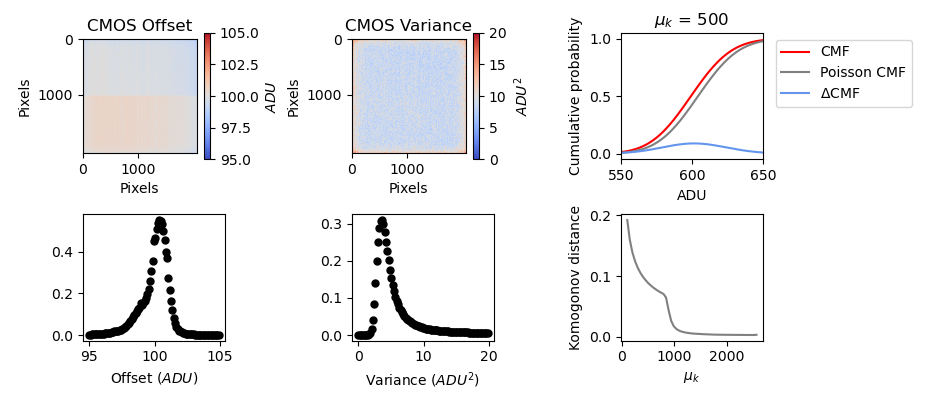
\includegraphics[width=16cm]{media/Noise.png}
\end{center}
\caption{\textbf{Noise calibration for a CMOS camera used for maximum-likelihood localization}. (left column) CMOS offset for zero incident photons (middle column) CMOS variance for zero incident photons (upper right) Cumulative mass function for the convolution distribution and its Poisson approximation for rate parameter $\mu_{k} = 500$ counts (lower right) Komogonov distance measured as a function of rate parameter $\mu_{k}$}
\label{fig:fig2}
\end{figure}

\begin{equation}
p(\bold{x}_{k}\lvert\theta) = A\sum_{q=0}^{\infty} \frac{1}{q!}e^{-\mu_{k}}\mu_{k}^{q}\frac{1}{\sqrt{2\pi}w_{k}}e^{-\frac{(\bold{x}_{k}-g_{k}q-o_{k})^2}{2 w_{k}^{2}}} \approx \mathrm{Poisson}(\mu_{k}')
\end{equation}

where $A$ is some normalization constant. For the sake of generality, we include a per-pixel gain factor $g_{k} \; [\mathrm{ADU}/\mathrm{photon}]$, which is often unity. Sampling from $p(\bold{x}_{k}\lvert\theta)$ is trivial; however, for computation of a lower bound on uncertainty in $\theta$, the summation can be difficult to work with. Therefore, we choose to use a Poisson approximation for simplification, valid under a range of experimental conditions \parencite{Huang2013}. The quality of this approximation will depend on the signal level, with higher signal levels or higher exposure times leading to a reduced Komogonov distance between the convolution distribution and the approximation (Figure \ref{fig:fig2}). After subtraction of the offset $o_{k}$ of the pixel array, the variance of the Poisson likelihood per pixel  becomes $\mu_{k}' = \mu_{k} + w_{k}^{2}$. Ultimately, the model negative log-likelihood is

\begin{equation}
\ell(\bold{x}\lvert\theta) = -\log \prod_{k} \frac{e^{-\left(\mu_{k}'\right)}\left(\mu_{k}'\right)^{n_{k}}}{n_{k}!} = \sum_{k}  \log n_{k}! + \mu_{k}' - n_{k}\log\left(\mu_{k}'\right)
\end{equation}

where $n_{k}$ is the number of ADU measured at pixel $k$. Localization then proceeds by optimization of $\ell(\bold{x}\lvert\theta)$ to obtain to maximum likelihood estimate (MLE) of the coordinates. 

\subsection{Cramer-Rao lower bound}

Reliable inference of $\theta$ from $\bold{x}$ in general requires performance metrics for model selection. Here, we use the Fisher information as an information theoretic criteria to assess the discrepancy between theoretical minimum precision with respect to the root mean squared error (RMSE) of our predictions of $\theta$, i.e. localization uncertainty \parencite{Chao2016}. The Poisson log-likelihood $\ell(\bold{x}\lvert\theta)$ is convenient for computing the Fisher information matrix \parencite{Smith2010} and thus, the Cramer-Rao lower bound (CRLB). This bounds the variance of a statistical estimator of $\theta$, from below: $\mathrm{var}(\hat{\theta}) \geq I^{-1}(\theta)$. The Fisher information is given by the expression

\begin{equation}
I_{ij}(\theta) = \underset{\theta}{\mathbb{E}}\left(\frac{\partial \ell}{\partial\theta_{i}}\frac{\partial\ell}{\partial\theta_{j}}\right) 
\end{equation}

For an arbitrary parameter, we find that, for a Poisson log-likelihood $\ell$:

\begin{align*}
\frac{\partial \ell}{\partial \theta_{i}} &= \frac{\partial}{\partial \theta_{i}} \sum_{k}  \log n_{k}! + \omega_{k}' - n_{k}\log\left(\omega_{k}'\right)\\
&= \sum_{k} \frac{\partial \omega_{k}'}{\partial\theta_{i}} \left(\frac{\omega_{k}'-n_{k}}{\omega_{k}'}\right)
\end{align*}

Using this result, we can compute the Fisher information matrix $I(\theta)$

\begin{equation}
I_{ij}(\theta) = \underset{\theta}{\mathbb{E}}\left(\sum_{k}\frac{\partial \omega_{k}'}{\partial\theta_{i}}\frac{\partial \omega_{k}'}{\partial\theta_{j}} \left(\frac{\omega_{k}'-n_{k}}{\omega_{k}'}\right)^{2}\right) = \sum_{k}\frac{1}{\omega_{k}'}\frac{\partial \omega_{k}'}{\partial\theta_{i}}\frac{\partial \omega_{k}'}{\partial\theta_{j}}
\end{equation}

A fundamental lower bound on the localization uncertainty in our estimates of $\theta$ then is found from its inverse: $\mathrm{CRLB} = I^{-1}(\theta)$.

\subsection{Maximization of density, minimization of error}

The distribution of a particular biomolecule in the cell can be described as a probability density over a two-dimensional space, casting super-resolution as a density estimation problem. Intuitively, the spatial resolution of SMLM images then increases as we draw more samples from this density, a concept which is made mathematically precise by the so-called Fourier ring correlation (FRC) \parencite{Nieuwenhuizen2013}. Using FRC, one can define image resolution as the spatial frequency at which a correlation function in the frequency domain drops below a threshold, typically taken to be $1/7$  (Figure \ref{fig:fig3}). This correlation function is defined for two concentric rings in the frequency domain:

\begin{figure}[t]
\begin{center}
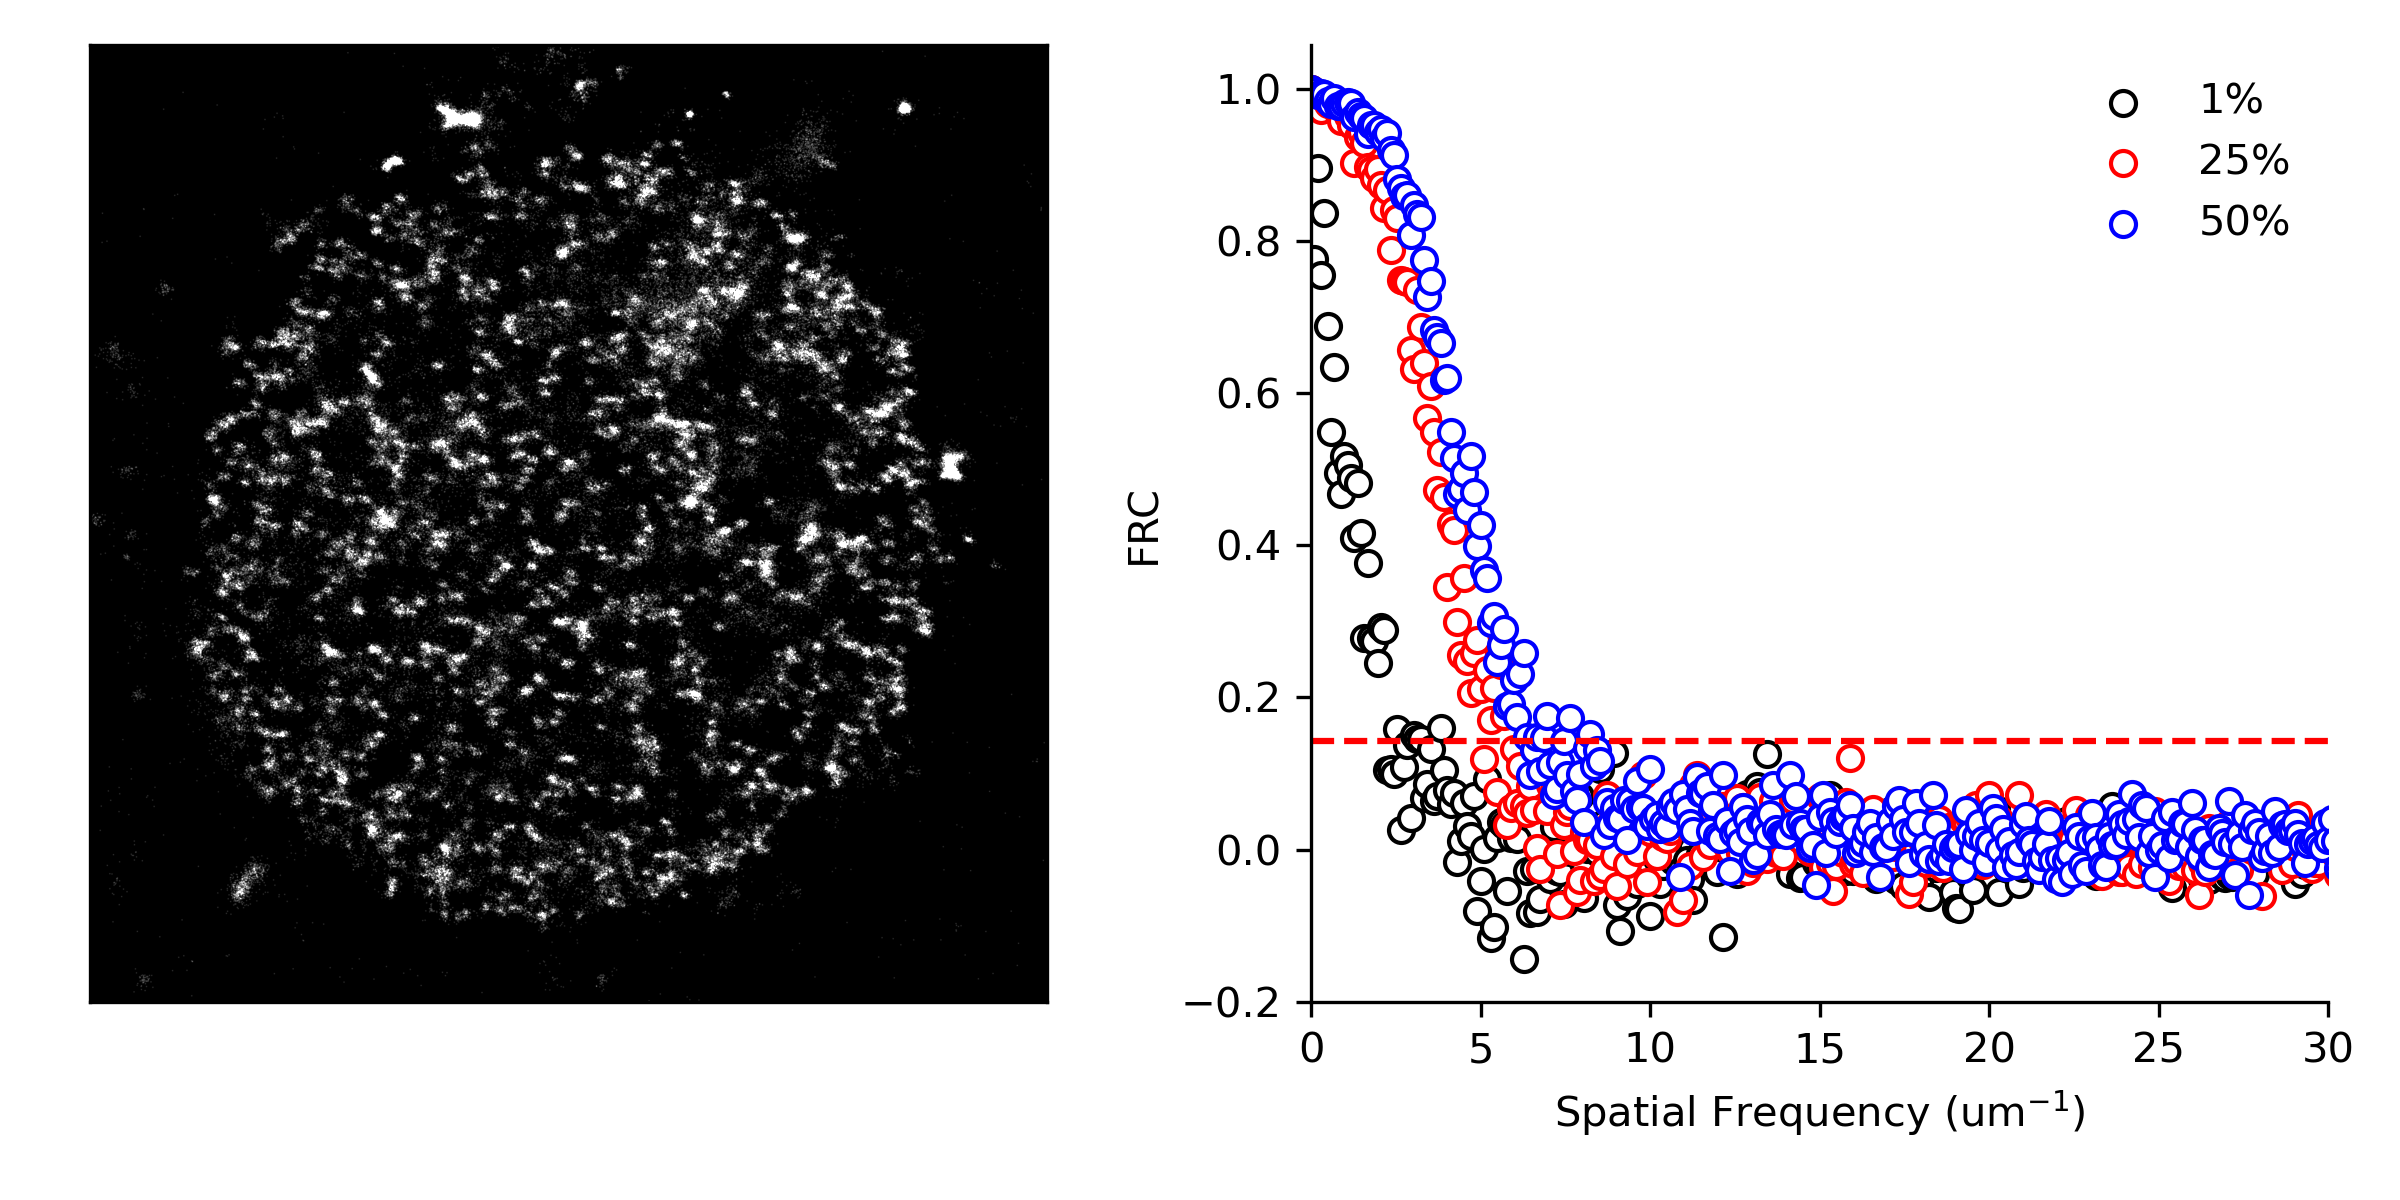
\includegraphics[width=10cm]{media/FRC.png}
\end{center}
\caption{\textbf{Resolution in nanoscopy depends on sampling density}. Fourier ring correlation (FRC) for different sampling ratios relative to an approximate total 200k localizations. (inset) Example kernel density estimate of H2B-HaloTag in a living HeLa cell nucleus. Scalebar approximately 5um}
\label{fig:fig3}
\end{figure}

\begin{equation}
\mathrm{FRC}(q) \vcentcolon = \frac{\sum_{\vec{q}\in\mathrm{ring}}\tilde{f_{1}}(\vec{q})\tilde{f_{2}}(\vec{q})^{*}}{\sqrt{\sum_{\vec{q}\in\mathrm{ring}}\lvert f_{1}(\vec{q})\lvert^{2}}\sqrt{\sum_{\vec{q}\in\mathrm{ring}}\lvert f_{2}}(\vec{q})\lvert^{2}}
\end{equation}

According to this theory, reducing localization uncertainty while increasing the number of samples, results in an increase in image resolution \parencite{Nieuwenhuizen2013}. However, typical nanoscopies favor fewer samples and lower localization uncertainty as few tools to deal with localization in dense scenes are available. Indeed, localization uncertainties in sparse conditions are often tens of nanometers and managing the increase in localization uncertainty at high labeling density remains a major bottleneck. Static uncertainty due to molecular crowding can be partially amelioriated by using pairwise or higher-order temporal correlations within a pixel neighborhood, known as stochastic optical fluctuation imaging (SOFI) \parencite{Dertinger2009}. Other approaches such as stimulated emission and depletion (STED) imaging bring control over the photophysical state of a chosen subset of the sample, yet the need for laser scanning prevents widespread application in live-cell studies. 

The spatial resolution and relative simplicity of nanoscopy techniques has incited an effort to increase their resolution, precision, and explore avenues towards time-resolved nanoscopy. In the next two chapters, we develop novel approaches to these issues which address localization in dense scenes as an inference problem in a high dimensional parameter space. In Chapter 2,  we leverage single photon avalanche diode (SPAD) arrays to count active fluorescent emitters which may lead to constrained multi-emitter localization using the image likelihood. SPAD cameras, with their high temporal resolution and single photon sensitivity, enable precise localization in non-sparse scenes. In Chapter 3, we design a generative modeling framework for kernel density estimation in localization microscopy, using variational diffusion. This approach not only accelerates super-resolution imaging but also provides a way to estimate uncertainty in the results. These two methods, one focusing on computational models and the other on cutting-edge hardware, offer complementary solutions to the high-dimensional inference problem in super-resolution microscopy. Using them separately or in tandem, we can achieve more accurate and reliable imaging of biological structures at the nanoscale. Finally, in Chapter 4, we apply a more conventional form of localization microscopy to the study of chromatin organization in living mammalian cells. 

